% !TEX encoding = UTF-8
% !TEX TS-program = pdflatex
% !TEX root = ../tesi.tex

%**************************************************************
\chapter{Progettazione e sviluppo}
\label{cap:progettazione}
%**************************************************************

\section{Progettazione}
\subsection{Architettura}

Prima di descrivere la varie aggiunte che sono state apportate al software, è necessario fornire un'idea dell'architettura sulla quale il progetto si basa. In questo modo si 
rendono più chiare molte delle scelte che sono state prese e il perché altre sono state scartate.\\ Di seguito è presentato uno schema ad alto livello di come sono strutturate le
varie componenti che formano l'intero sistema. Come possiamo notare in \hyperref[4.1]{Figura 4.1}, il progetto segue un flusso pressoché "ciclico", partendo dal recupero dei dati dal
database e infine fornendo la soluzione. I dati estratti dal database vengono convertiti in file JSON il quale verrà letto dall'algoritmo che ha il compito di trovare la soluzione,
una volta fornita la soluzione essa viene ritradotta in un file JSON il quale viene letto e trasposto nell'interfaccia utente.

\begin{figure}[H]
	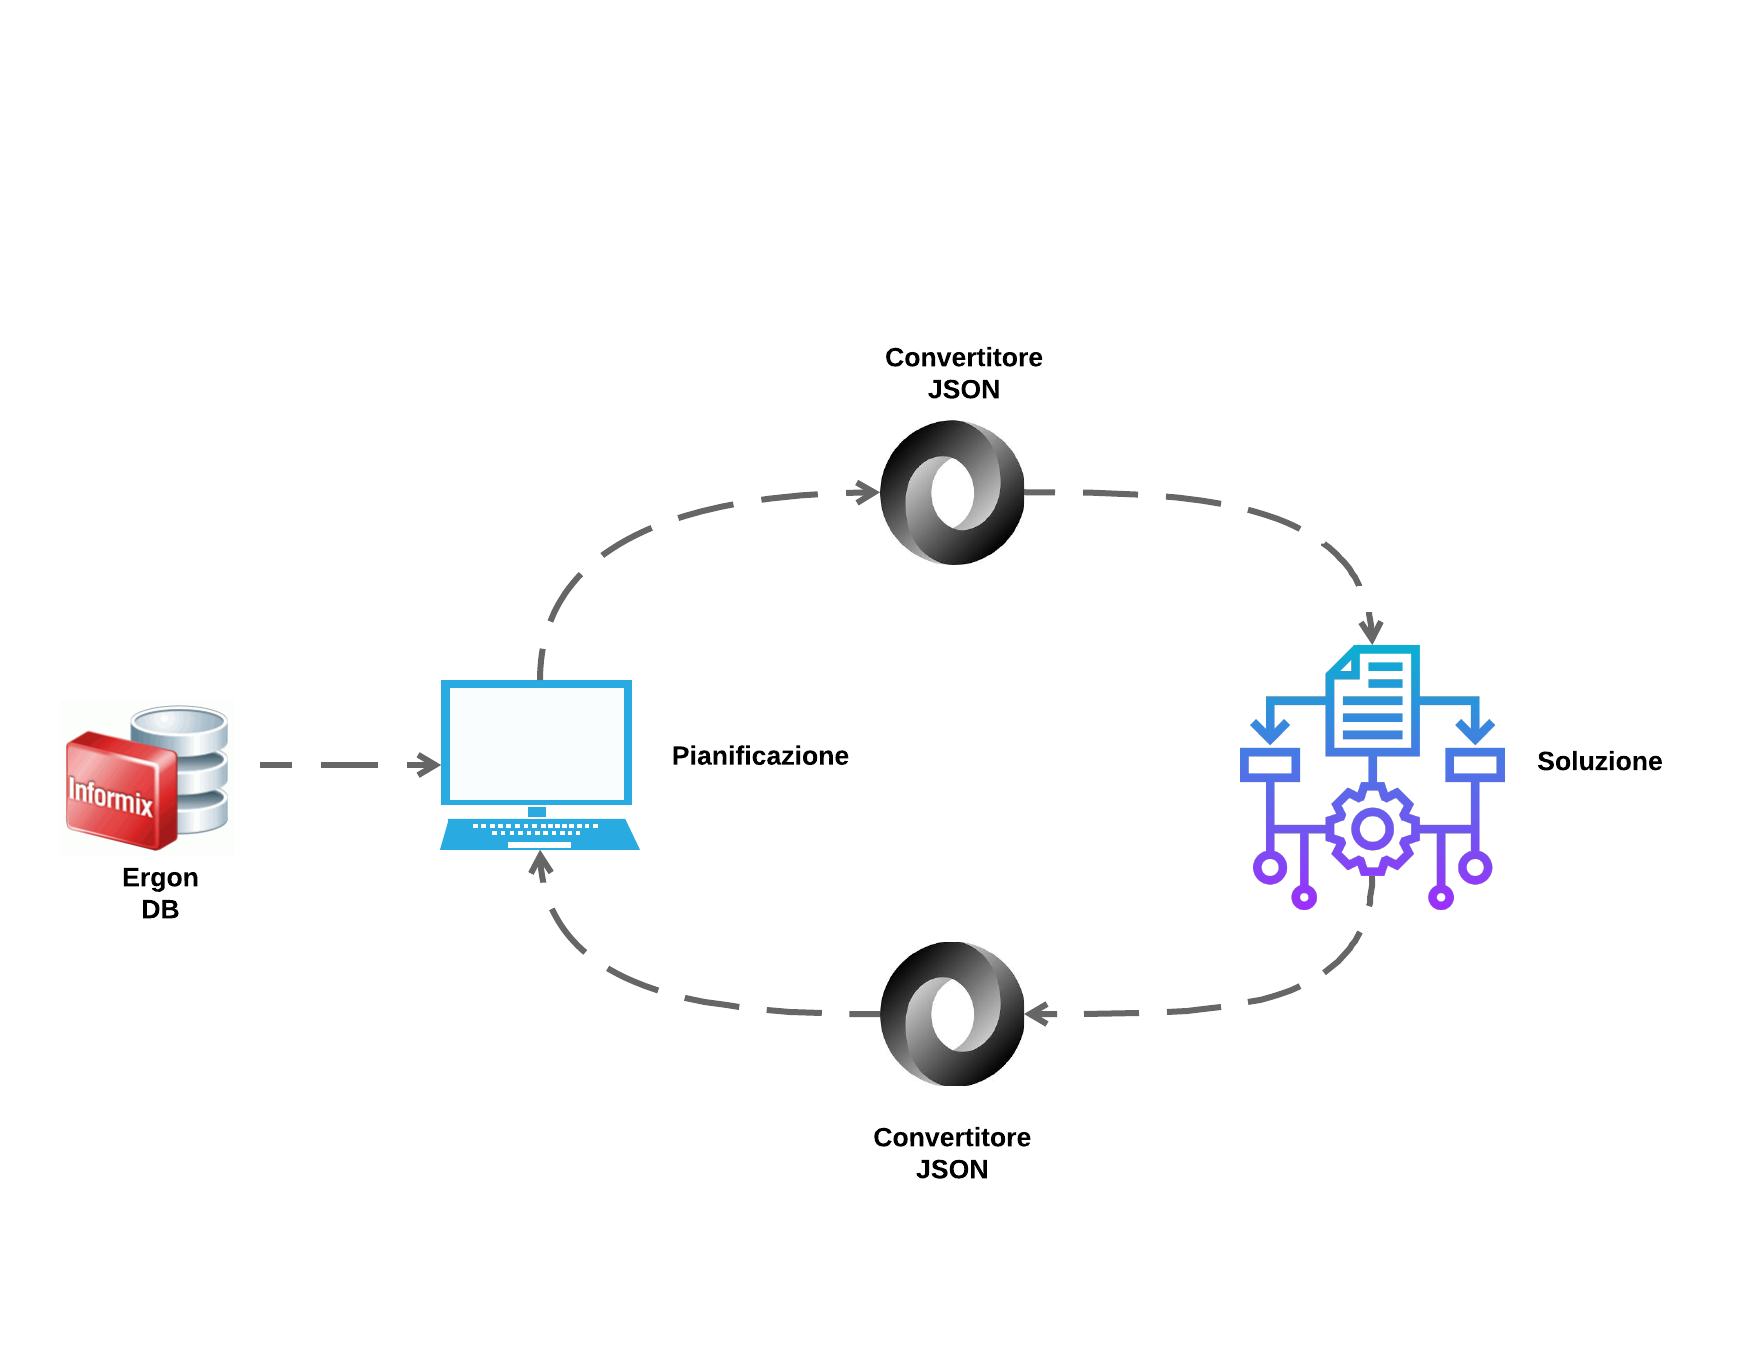
\includegraphics[width=13cm]{immagini/architettura.png}
	\centering
    \caption{Architettura generale}
    \label{4.1}
\end{figure}

\subsection{Algoritmo}

\textbf{Il problema}

Il problema della pianificazione della produzione rientra nella categoria \hyperref[Np-hard]{NP-hard\glo} in quanto è riconducibile al problema del 
\hyperref[Commesso viaggiatore]{commesso viaggiatore\glo} \hyperref[slide]{[15]}. 
In aggiunta al problema del commesso viaggiatore si devono considerare
altri vincoli come: 
\begin{itemize}
    \item tempo massimo sul quale si vogliono pianificare gli ordini;
    \item numero di linee sulle quali si possono produrre determinati ordini;
    \item vincoli generali di sequenza che andremo a definire in seguito.
\end{itemize}

Queste caratteristiche avevano portato, nella precedente fase del progetto, a optare per lo sviluppo di algoritmi di soluzione \hyperref[slide]{euristici\glo [15]}.
Con la richiesta di estendere tale progetto, il numero di vincoli da soddisfare cresce in proporzione al numero di ordini che si vogliono pianificare.
In particolare vanno tenuti in considerazione i vincoli precedenti più l'aggiunta dei seguenti:

\begin{itemize}
    \item pianificazione dei semilavorati antecedente ai prodotti finiti;
    \item materie prime e semilavorati presenti in quantità sufficienti per la produzione;
    \item verifica della disponibilità di materie prime e semilavorati in base agli ordini fornitori.
\end{itemize}

In conclusione, il problema che il progetto si pone di risolvere, consiste nel trovare una soluzione ammissibile \hyperref[slide0]{[16]}, quanto più vicina all'ottimo,
della pianificazione
in base ai vincoli imposti.\newline

\textbf{La soluzione}

Dovendo appoggiarsi all'algoritmo esistente, non è stato possibile eseguire uno stravolgimento completo del suo funzionamento, anzi si è cercato di inserire le nuove funzionalità
in modo da integrarle il più possibile, senza effettuare modifiche sostanziali, alla struttura del codice esistente.\\ Per fare ciò, si è fatto ampio uso di nuove funzioni e
classi, in modo da garantire un alto grado di modularità del codice aggiunto a quello esistente.
\\ La struttura di partenza sulla quale vengono integrati i nuovi moduli è composta da una fase iniziale
di lettura dei dati dal database. Tali dati vengono convertiti in un file JSON che, per comodità di esecuzione, viene letto nuovamente dallo stesso programma, anche se
l'dea di base sarebbe quella di delegare la sua lettura e successiva elaborazione dei dati ad un sistema centralizzato esterno all'azienda che fornisce i dati stessi.\\
Una volta ottenuti i dati in formato JSON, vengono inseriti nell'algoritmo tramite l'impiego di classi e strutture predisposte. Tali classi vengono utilizzate come parametri
per la prima funzione che si pone come obiettivo quello di fornire una soluzione ammissibile nel minor tempo possibile attraverso un algoritmo \hyperref[Greedy]{Greedy\glo}.\\
Tale algoritmo ha il compito di valutare, in modo sequenziale, i vari ordini che necessitano di essere pianificati, se un ordine soddisfa i vincoli imposti allora verrà inserito nella soluzione iniziale.
Una volta ottenuta la soluzione iniziale, questa viene fornita alla successiva funzione di ottimizzazione, composta da un algoritmo di \hyperref[Tabu Search]{Tabu Search\glo}. Tale algoritmo ha il compito
di eseguire un insieme di mosse specifiche in modo casuale, valutando di volta in volta la bontà della soluzione ottenuta dopo la loro esecuzione. Al termine di un numero prefissato
di iterazioni, o dopo aver soddisfatto i criteri di terminazione, verrà fornita la soluzione "ottimizzata" da visualizzare.\\
Di seguito viene illustrato il funzionamento degli algoritmi adottati, ottenuti dall'integrazione dei precedenti algoritmi.\\

\textbf{Algoritmo Greedy}

L'algoritmo Greedy \hyperref[slide]{[15]} è il primo passo per ottenere una soluzione ammissibile del problema in questione. Tale algoritmo è sviluppato tenendo in considerazione che non è possibile effettuare dei "passi indietro",
ovvero, una volta inserito un ordine in pianificazione tale ordine rimane fino alla fine dell'esecuzione. I parametri in ingresso di tale algoritmo sono i seguenti:
\begin{itemize}
    \item ordini da pianificare;
    \item materie prime e semilavorati presenti in magazzino;
    \item materie prime e semilavorati presenti in ordini fornitori;
    \item linee di lavorazione con i rispettivi vincoli.
\end{itemize}

L'ordine di funzionamento è quindi il seguente:

\begin{itemize}
    \item prima scelta \hyperref[Euristica]{euristica\glo}, vengono ordinati i prodotti in base alla loro data di spedizione;
    \item il primo ordine in questione viene valutato;
    \item si verifica la presenza di materie prime, e qui abbiamo i seguenti casi:
            \begin{itemize}
                \item le materie prime sono disponibili per produrre l'ordine, inserisco in pianificazione;
                \item le materie prime non sono disponibili per produrre l'ordine, verifico l'arrivo di eventuali materie prime da parte dei fornitori,
                 se ciò avviene inserisco in pianificazione;
                \item non pianifico l'ordine.
            \end{itemize}
    \item si verifica la presenza di semilavorati, e qui abbiamo i seguenti casi:
            \begin{itemize}
                \item i semilavorati sono disponibili per produrre l'ordine, inserisco in pianificazione;
                \item i semilavorati non sono disponibili per produrre l'ordine, provo ad eseguire la pianificazione dei semilavorati mancanti, se ciò avviene
                inserisco in pianificazione;
                \item non pianifico l'ordine.
            \end{itemize}
    \item ogni valutazione effettua un controllo se è possibile inserire l'ordine in base al tempo lavorativo rimanente;
    \item si ripetono le azioni sopracitate fino al termine della valutazione di tutti gli ordini da pianificare.
\end{itemize}

Si ricorda che non è necessario che tutti gli ordini richiesti siano inseriti nella pianificazione, in quanto uno dei precedenti vincoli può non essere soddisfatto e, se tale ordine venisse
inserito nella soluzione, quest'ultima sarebbe non ammissibile perché viola appunto almeno uno dei vincoli imposti. Inoltre, se si esegue un accurato controllo, si può notare che 
il risultato fornito al termine della sua esecuzione, in alcuni casi, ha un ampio margine di miglioramento. L'algoritmo Greedy ha come obiettivo quello di creare una
soluzione iniziale nel modo più rapido possibile, in modo da ottenere una base di partenza per la successiva ottimizzazione eseguita dall'algoritmo Tabu Search.\\


\textbf{Tabu Search}

Una volta ottenuta la prima soluzione ammissibile, fornita dall'algoritmo Greedy, l'esecuzione si sposta sulla sua ottimizzazione tramite la Tabu Search \hyperref[tabu]{[17]}.
Questa particolare tecnica meta-euristica ha lo scopo di fornire una soluzione\hyperref[scheduling]{[18]}, più vicina all'ottimo, tramite l'esecuzione di mosse che perturbano
la soluzione corrente alla ricerca iterativa di soluzioni sempre migliori. L'esecuzione di queste mosse in modo casuale porta ogni volta ad una nuova soluzione ammissibile, tale risultato viene poi confrontato con la soluzione
precedente, se il risultato è migliorativo allora verrà considerato come nuova miglior soluzione e si utilizzerà per la successiva iterazione, altrimenti tale risultato 
verrà semplicemente scartato e si prosegue con l'esecuzione della mossa successiva. Di seguito è presentato l'ordine di funzionamento di tale algoritmo:
\begin{enumerate}
    \item selezione casuale della mossa da eseguire tra le seguenti:
    \begin{itemize}
        \item mossa aggiungi articolo;
        \item mossa sposta articolo;
        \item mossa scambia articoli;
        \item mossa elimina articolo;
        \item mossa sposta sequenza; 
        \item mossa scambia sequenza.  
    \end{itemize}
    \item validazione della mossa scelta, tramite l'utilizzo della \hyperref[Tabu List]{Tabu List\glo} \hyperref[list]{[19]};
    \item esecuzione della mossa scelta;
    \item valutazione della nuova soluzione in rapporto con la soluzione precedente;
    \item viene ripetuta l'esecuzione nell'ordine sopracitato fino al termine del numero massimo di iterazioni, del tempo imposto o del soddisfacimento di uno dei criteri di
    terminazione.\\
\end{enumerate}


\textit{Scelta della mossa}\\
È utile entrare maggiormente nel dettaglio dei punti precedenti per avere un'idea di come si ottiene la soluzione ottimizzata.\\
Al punto uno, la scelta della mossa, viene eseguita in modo casuale. Durante lo stage, la scelta casuale è stata integrata attraverso l'impiego di alcuni metodi di \hyperref[Diversificazione]{diversificazione\glo} o \hyperref[Intensificazione]{intensificazione\glo}. 
In modo da "forzare" la successiva mossa da scegliere,
quindi non rendendola più completamente casuale. Nel caso dell'intensificazione si punta a scegliere l'insieme di mosse che, ad esempio, nelle loro esecuzioni precedenti hanno fornito
risultati migliori e quindi si pensa potranno fornire migliori risultati anche in futuro, in questo modo ci si concentra maggiormente su queste scartando le altre.\\
Al contrario, la diversificazione può decidere di eseguire le mosse che sono state meno eseguite in precedenza così da indirizzare i risultati verso strade mai 
percorse.\\ È proprio quest'ultimo caso che, a seguito di una discussione con il tutor aziendale, è stato inserito nel programma esistente. Il suo funzionamento è semplice ma non banale:
dopo l'esecuzione di metà delle iterazioni concesse alla Tabu Search entra in gioco tale meccanismo, si è deciso di considerare l'esatta metà così da poter ottenere inizialmente una
soluzione meno forzata possibile, da tale momento in poi verrà assegnato un peso percentuale ad ogni mossa che diminuirà ad ogni esecuzione della stessa, aumentando quindi il 
peso delle rimanenti.\\ 
Si è scelto di utilizzare questo metodo per poter garantire comunque un alto grado di casualità, criterio che, nel precedente algoritmo, si è rivelato importante per le prestazioni.\\

\textit{Validazione della mossa scelta}\\
Anche in questo caso è utile approfondire come avviene la validazione di una mossa scelta in modo casuale. In particolare, in alcuni casi, possiamo direttamente scartare
l'esecuzione della mossa perché siamo sicuri che porterà ad una soluzione non migliorativa.\\ Ogni algoritmo di Tabu Search fa affidamento su una relativa 
Tabu List , la quale non è altro che uno storico delle mosse eseguite in precedenza, le quali non dovranno essere rieseguite, almeno nell'immediato futuro.\\
Un criterio importante da tenere presente
è la lunghezza che si sceglie di dare a tale lista, questo perché una lista troppo corta non garantisce che non vengano eseguite mosse utilizzate da poco tempo, mentre, una 
lista troppo lunga tende a creare troppa diversificazione delle soluzioni.\\ Nel progetto di stage alla Tabu List veniva aggiunta anche la mossa opposta a quella eseguita, in modo
da salvare sia la mossa che ha portato ad una nuova soluzione, sia la sua mossa opposta, evitando così di tornare casualmente alla soluzione precedente. 
La validazione di una mossa,
in seguito, deve inoltre sottostare a dei vincoli che appartengono alla realtà sulla quale si basa il nostro applicativo. Ad esempio, se viene considerata la mossa \textit{aggiungi articolo}
ma non abbiamo nessun articolo da aggiungere, tale mossa viene scartata.\\ Con l'aggiunta della pianificazione dei semilavorati, i quali ricordiamo avere le stesse peculiarità
dei prodotti finiti, sono stati aggiunti ulteriori controlli, in quanto non possiamo garantire l'eliminazione tramite la mossa \textit{elimina articolo} di uno di questi senza
eliminare anche l'articolo a cui fanno riferimento.\\ Perciò si è scelto di eseguire l'eliminazione solo sui prodotti finiti. Altri controlli da eseguire riguardano lo spostamento
di articoli o sequenze, nel caso venga selezionato lo spostamento di un semilavorato bisogna accertarsi che non venga inserito in pianificazione successivamente al relativo
prodotto finito. Allo stesso modo è stato necessario aggiungere controlli sulla giacenza e sull'arrivo di merci dai fornitori, questo perché lo spostamento, l'eliminazione e l'aggiunta
di articoli creava una forte oscillazione nei dati riguardanti i materiali da lavorazione e spesso riconduceva ad una soluzione peggiorativa.\\ Come si può intuire, l'aggiunta
di tutti questi vincoli ha minato la capacità di ottenere una soluzione nettamente migliorativa da parte della Tabu Search.\\

\textit{Esecuzione della mossa scelta}\\
Una volta accertati che la mossa sia eseguibile si passa alla sua implementazione.\\ Ogni mossa è correlata ad un insieme di funzioni che hanno il compito di accertarsi che ad
ogni passo della sua esecuzione ci si trovi all'interno di una soluzione ammissibile. È facile riscontrare che, durante l'esecuzione di una di queste mosse, si possa terminare 
in una soluzione non ammissibile, in questo caso viene scartato il nuovo risultato e si torna alla soluzione ammissibile precedente.\\ Nel caso in cui siano soddisfatti tutti
i vincoli imposti al termine dell'esecuzione di una mossa la soluzione ottenuta sarà ammissibile e sarà compito del prossimo passo dell'algoritmo accertarne la bontà.\\

\textit{Valutazione della soluzione}

Una volta ottenuta un nuova soluzione è necessario valutarla per sapere se sia migliorativa o peggiorativa rispetto alla precedente.\\
Il confronto quindi viene eseguito calcolando il punteggio della nuova soluzione il quale è dato dalla seguente funzione:
%\[F(s) = \frac{Pz}{Pz\ped{tot}}*Peso\ped{pz} - \frac{T\ped{linee}}{T\ped{linee-tot}}*Peso\ped{pz}\]

\[\frac{\text{Pezzi pianificati}}{\text{Totale pezzi richiesti}} \times \text{Peso del rapporto pezzi}\]\\

Qui otteniamo il punteggio di maggior spessore, dal quale si sottraggono i seguenti:

\[\frac{\text{Occupazione linee}}{\text{Massima occupazione linee}} \times \text{Peso del rapporto occupazione}\]\\

\[\frac{\text{Tempo totale di pianificazione}}{\text{Massimo tempo a disposizione}} \times \text{Peso del rapporto tempo}\]\\

Una volta ottenuto il relativo punteggio viene eseguito il confronto con la soluzione precedente e si sceglie la soluzione avente il punteggio più alto.\\
Questo non è l'unico metodo con il quale si sceglie la soluzione che riteniamo essere migliore.\\ Vengono impiegati dei criteri di \hyperref[Criteri di aspirazione]{aspirazione\glo} i quali hanno il compito
di valutare anche soluzioni che hanno punteggi inferiori alla precedente ma che potrebbero essere un buon punto di partenza per la valutazione di soluzioni successive.\\
Nel progetto è stato inserito un criterio di aspirazione con il seguente funzionamento: se la nuova soluzione ha un punteggio inferiore alla soluzione precedente, ma il 
numero di pezzi prodotti è superiore, allora se la differenza è inferiore al 2\% la nuova soluzione è considerata migliore. Questo perché lo scopo ultimo della pianificazione
è riuscire a pianificare il maggior numero di ordini possibili.


\subsection{Codifica}

In questa sezione vengono illustrati i vari passi seguiti durante la fase di codifica del progetto, specificando i punti fondamentali di ognuno.\\

\title{Implementazione controllo giacenze}

Il primo obiettivo da raggiungere riguardava l'esecuzione della pianificazione in base alle materie prime e semilavorati presenti in magazzino.
Per fare ciò, sono stati eseguiti i passi presentati di seguito:\\ \\
\textbf{Controllo giacenze}
\begin{enumerate}
        \item lettura dal database dei dati riguardanti le giacenze;
        \item utilizzo di una funzione di esplosione distinta per ottenere la \hyperref[Distinta base]{distinta base\glo} dei prodotti finiti; 
        \item scrittura dei dati in un file JSON;
        \item creazione di una classe volta a lavorare sulle giacenze;
        \item creazione di una funzione volta al controllo della presenza di materiali per eseguire la pianificazione;
        \item integrazione di tale funzione con gli algoritmi Greedy e Tabu Search;
        \item rimozione dei materiali necessari a produrre un prodotto finito;
        \item reintegrazione dei materiali in magazzino se uno o più articoli vengono eliminati dalla pianificazione.\\
\end{enumerate}

\textbf{Pianificazione semilavorati} 
\begin{enumerate}
        \item utilizzo di una funzione di esplosione distinta per ottenere la distinta base dei prodotti finiti; 
        \item scrittura dei dati in un file JSON;
        \item riutilizzo della classe \textit{Ordine} per i semilavorati;
        \item ampliamento delle funzionalità della classe \textit{Ordine} per tenere traccia dei semilavorati di ogni prodotto finito;
        \item integrazione della pianificazione dei semilavorati nell'algoritmo Greedy, anticipando la loro produzione rispetto al prodotto finito;
        \item inserimento di controlli ausiliari per impedire spostamenti ed eliminazioni durante l'esecuzione dell'algoritmo di Tabu Search.\\
\end{enumerate}

In \hyperref[pian-semilavorati]{Figura 4.2} è mostrato come si presenta la pianificazione restituita dall'applicativo dopo la pianificazione dei semilavorati.

\begin{figure}[H]
	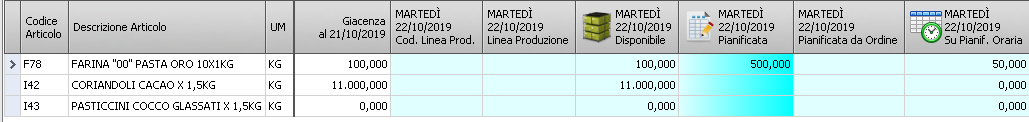
\includegraphics[width=\textwidth]{immagini/sl_planning.png}
	\centering
\end{figure}
\begin{figure}[H]
	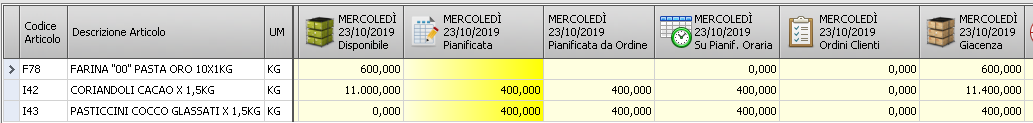
\includegraphics[width=\textwidth]{immagini/sl_planning2.png}
    \centering
    \caption{Pianificazione semilavorati}
    \label{pian-semilavorati}
\end{figure}

Dalla \hyperref[pian-semilavorati]{Figura 4.2} vediamo che \textit{F78} è un semilavorato, di cui abbiamo 100kg in giacenza, richiesto dai prodotti finiti \textit{I42} e \textit{I43}.\\
Sappiamo che i due prodotti finiti in questione richiedono 300kg del semilavorato \textit{F78} ciascuno, e vediamo che il martedì ne sono pianificati esattamente 500kg
per garantire la produzione di \textit{I42} e \textit{I43} il mercoledì.

\newpage

\textbf{Controllo ordini fornitori} 
\begin{enumerate}
        \item lettura dal database i dati riguardanti gli ordini fornitori; 
        \item scrittura dei dati in un file JSON;
        \item creazione di una classe volta a lavorare sugli ordini fornitori;
        \item ampliamento della funzione dedita al controllo delle giacenze;
        \item integrazione di tale funzione con gli algoritmi Greedy e Tabu Search;
        \item inserimento di controlli ausiliari per evitare di ottenere soluzioni non ammissibili durante l'esecuzione di entrambi gli algoritmi.\\
\end{enumerate}

\textbf{Pianificazione ordini da magazzino} 
\begin{enumerate}
        \item lettura di ordini da inserire in pianificazione direttamente dal magazzino;
        \item scrittura dei dati in un file JSON;
        \item riutilizzo della classe \textit{Ordine} per gli ordini da magazzino;
        \item utilizzo di tutti i vincoli precedenti per effettuare la pianificazione.\\
\end{enumerate}

\textbf{Criteri di Diversificazione/Intensificazione}\\ 

Per ottenere il massimo dall'esecuzione dell'algoritmo di Tabu Search, si è infine scelto di utilizzare una tecnica di diversificazione come spiegato nella sezione precedente \hyperref[criteria]{[20]}.

\newpage

\section{Verifica e validazione}

La fase di verifica si è protratta durante tutta la fase di sviluppo del progetto. Sono state impiegate delle tecniche di analisi statica, in quanto non era previsto un piano di test
da effettuare sui risultati ottenuti.\\ Il non eseguire dei test automatici sui risultati ottenuti deriva anche dal fatto che i dati utilizzati corrispondano
a dei dati reali, per i quali sarebbe stato più complicato codificare un insieme di test automatici. La problematica precedente avrebbe sottratto un considerevole ammontare di tempo allo sviluppo del
codice applicativo. 

\subsection{Analisi statica}

Si è fatto ampio uso dello strumento di debug fornito da Visual Studio 2010 e ho creato una lista di controllo tramite \hyperref[Breakpoint]{breakpoint\glo} in modo da poter
valutare, durante l'esecuzione, lo stato del software ad ogni punto critico. Ciò ha permesso di individuare efficacemente gli errori a livello logico che si sono presentati
durante la varie fasi di sviluppo. Si è proseguito poi con dei controlli a campione della soluzione presentata a video dal programma, 
valutando determinati ordini, in modo da ottenere un riscontro reale della bontà della soluzione stessa. 

\subsection{Analisi dinamica}

Si è fatto uso di più funzioni con il compito di attestare che la soluzione corrente sia ammissibile, in particolare ogni funzione aveva il compito di verificare che
determinati vincoli fossero rispettati. Ad esempio, dopo aver inserito il controllo sulle materie prime e semilavorati, veniva verificato che la rimozione di queste due componenti
combaciasse con quanto risultava presente in magazzino. Sono stati effettuati altri controlli sul tempo di pianificazione rimanente e vincoli di linea imposti dalle relative
aziende. Si sottolinea che queste funzioni vengono richiamate solo in punti ben definiti nel codice, in quanto non sarebbe utile richiamare la stessa funzione di controllo
se i vincoli che attesta non sono stati modificati nella soluzione. Nel caso in cui una di queste funzioni accertasse l'inammissibilità della soluzione corrente veniva 
lanciata un eccezione, la quale riportava il vincolo che non era stato soddisfatto.


\subsection{Validazione}

Al raggiungimento di ogni stato rilevante dell'applicativo veniva eseguito un collaudo. Questo aveva il compito di accertare che i risultati ottenuti fossero in linea con
quanto ci si aspetta dalla pianificazione reale. Per fare ciò si eseguiva l'applicativo con i dati reali di una specifica azienda, dei quali si era giunti ad ottenere
una soluzione relativamente buona. Una volta confrontate le due soluzioni evidenziavo le eventuali discrepanze e passavo ad una verifica accurata di quanto ottenuto.
Seguiva poi una discussione con il tutor interno per accertarsi che tali scostamenti derivassero dalle nuove aggiunte e non fossero errori logici del programma.\\ Una volta 
accertati che la soluzione ottenuta fosse ammissibile e coerente veniva salvata e impiegata nelle successive fasi di validazione e collaudo.

\section{Risultati dei test}

Di seguito vengono riportati i risultati sui test effettuati durante le varie fasi di sviluppo del progetto. Sono presentati in forma grafica così da garantire un'immediata
comprensione.\\ I dati utilizzati per ottenere questi risultati fanno parte degli ordini, delle giacenze di magazzino 
e degli ordini fornitori di uno specifico cliente di Ergon Informatica.\\
Ogni test è stato effettuato sullo stesso ammontare di ordini distribuito in una singola settimana lavorativa, questo per garantire una continuità tra i vari test eseguiti.\\
L'insieme dei dati utilizzati sono i seguenti:
\begin{itemize}
    \item Numero ordini = 273;
    \item Numero semilavorati = 183;
    \item Numero giacenze = 525;
    \item Numero ordini fornitori = 57.
\end{itemize}

Si precisa che non tutti gli ordini devono essere pianificati e che vengono presi in considerazione solo i dati riguardanti la settimana corrente di pianificazione.
Ogni grafico è presentato in due diverse versioni, una tramite grafico a barre per confrontare le diverse misurazioni e una tramite grafico a dispersione per evidenziare
l'andamento della soluzione.
\subsection{Pianificazione prodotti finiti}

In \hyperref[4.3]{Figura 4.3} viene rappresentato l'andamento temporale dell'esecuzione dell'algoritmo Greedy e Tabu Search al variare del numero di iterazione massime consentite.

\begin{figure}[H]
	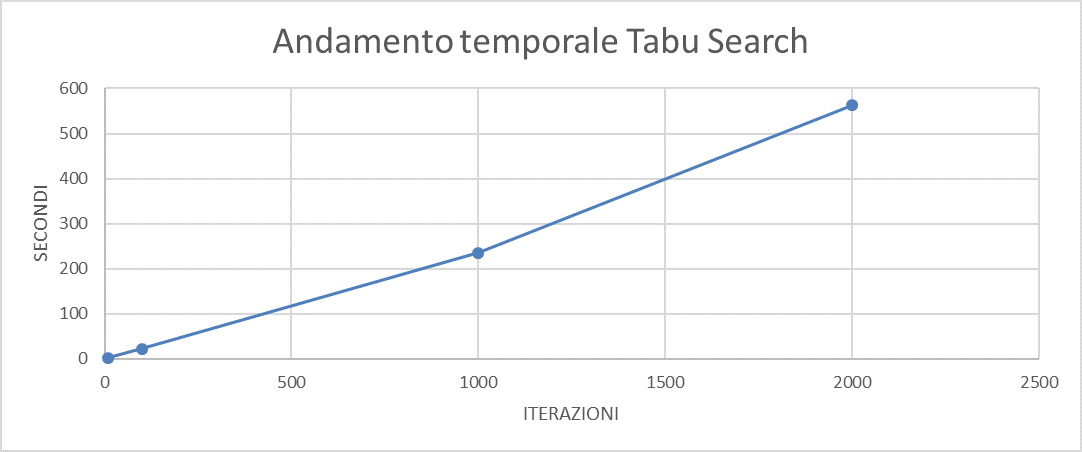
\includegraphics[width=13cm]{immagini/graficoPF2.png}
	\centering
	\caption{Grafico temporale della pianificazione dei prodotti finiti}
    \label{4.3}
\end{figure}

Per quanto riguarda il tempo di esecuzione dell'algoritmo Tabu Search vediamo un aumento in proporzione al variare del numero di iterazioni.
In \hyperref[4.4]{Figura 4.4} viene mostrato il miglioramento in percentuale, rispetto alla soluzione fornita dall'algoritmo Greedy, ottenuto dall'algoritmo di ottimizzazione.

\begin{figure}[H]
	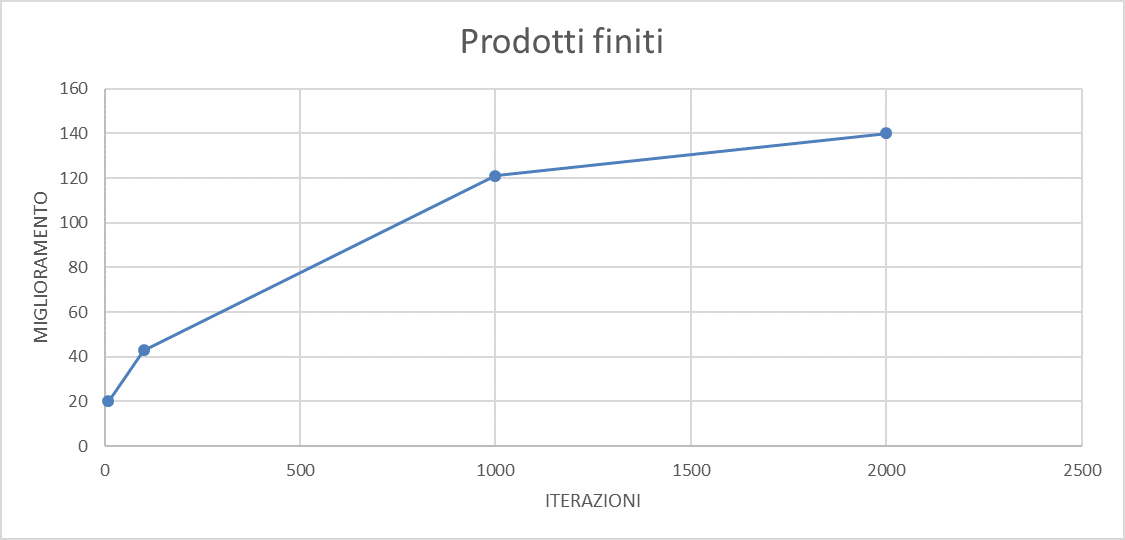
\includegraphics[width=13cm]{immagini/graficoPF3.png}
	\centering
    \caption{Grafico miglioramento percentuale della soluzione della pianificazione dei prodotti finiti}
    \label{4.4}
\end{figure}

Dopo vari test eseguiti posso affermare che, considerando anche il tempo impiegato, il numero di iterazioni ideale si assesti tra le 1000 e 2000 iterazioni.
Superate le 2000 iterazioni il miglioramento assume un andamento asintotico ed evidenzia solo uno spreco di tempo di esecuzione. 

\newpage
\subsection{Pianificazione semilavorati}

In \hyperref[4.5]{Figura 4.5} sono rappresentati i risultati dei test eseguiti dopo il primo importante avanzamento del progetto ovvero la pianificazione dei semilavorati.

\begin{figure}[H]
	\includegraphics[width=13cm]{immagini/graficosl2.png}
	\centering
    \caption{Grafico temporale con aggiunta della pianificazione dei semilavorati}
    \label{4.5}
\end{figure}

La prima cosa da notare è l'aumento del tempo di esecuzione da parte dell'algoritmo Greedy, il quale necessita ora di un elevato numero di controlli aggiuntivi. La funzione
stessa è stata resa \hyperref[Ricorsione]{ricorsiva\glo} in modo da riutilizzare il codice al suo interno per eseguire la pianificazione dei semilavorati. Questo ha permesso anche di creare una
relazione diretta tra il semilavorato e il suo prodotto finito, il tutto tramite una relazione padre figlio creata appositamente nella classe.
In compenso, l'algoritmo di Tabu Search non ha subito un aumento considerevole del tempo di esecuzione ma ha subito un calo drastico nella capacità di ottimizzazione della
soluzione.

\begin{figure}[H]
	\includegraphics[width=13cm]{immagini/graficosl3.png}
	\centering
    \caption{Grafico miglioramento percentuale della soluzione della pianificazione dei semilavorati}
    \label{4.6}
\end{figure}

Come possiamo notare in \hyperref[4.6]{Figura 4.6}, al termine delle 2000 iterazioni, il fattore di miglioramento si aggira attorno 19\%. Questo è dovuto al fatto che l'algoritmo
si trova di fronte a un elevato numero di controlli ausiliari prima di poter eseguire una mossa. Si prenda ad esempio la mossa di eliminazione, non può essere effettuata su un semilavorato
per questioni logico/reali in quanto non sarebbe più possibile pianificare il suo prodotto finito relativo. Allo stesso modo non è possibile spostare la pianificazione di un
semilavorato successivamente al suo prodotto finito e viceversa non è possibile pianificare il prodotto finito prima dei suoi semilavorati. Ciò è la causa della perdita di
capacità di ottimizzare la soluzione ottenuta dall'algoritmo Greedy.

\newpage
\subsection{Controllo ordini fornitori}

In aggiunta alla pianificazione dei semilavorati, è stato aggiunto il controllo sull'arrivo di materiale da parte dei fornitori.\\Ciò permette di non scartare a priori la possibilità
di pianificare alcuni ordini che, a causa dell'assenza di materiali, non verrebbero considerati. In questo modo, vengono considerati pianificabili tutti gli ordini per i quali
è presente almeno un ordine fornitore che soddisfa la quantità di materiali necessari. 

\begin{figure}[H]
	\includegraphics[width=13cm]{immagini/graficofo2.png}
	\centering
    \caption{Grafico temporale con aggiunta della pianificazione degli ordini fornitori}
    \label{4.7}
\end{figure}

Come si può notare in \hyperref[4.7]{Figura 4.7} la Tabu Search, anche in questo caso, impiega più tempo al variare del numero di iterazioni, ma rimanendo comunque entro limiti accettabili.

\begin{figure}[H]
	\includegraphics[width=13cm]{immagini/graficofo3.png}
	\centering
    \caption{Grafico miglioramento percentuale della soluzione della pianificazione degli ordini fornitori}
    \label{4.8}
\end{figure}

Dalla \hyperref[4.8]{Figura 4.8} si evince la netta incapacità della Tabu Search di ottenere una soluzione migliore partendo dalla soluzione fornita dall'algoritmo Greedy.\\
Questo avviene perché, in questo caso particolare, molti ordini sarebbero pianificabili per quanto riguarda i materiali a disposizione (cosa non realizzabile per le fasi
precedenti) e questo va a diminuire nettamente il risultato del rapporto pesato \[\frac{\text{Pezzi pianificati}}{\text{Totale pezzi richiesti}} \times \text{Peso del rapporto pezzi}\]\\
dove in \textit{Totale pezzi richiesti} vengono considerati tutti gli ordini producibili.\\ Inoltre, avendo un grandissimo numero di ordini producibili, le mosse eseguite 
dalla Tabu Search non fanno altro che sostituire ordini con altri ordini quindi non può ottenere un miglioramento significativo. Viene presentato in \hyperref[4.9]{Figura 4.9} 
il riassunto dei risultati ottenuti riguardanti il miglioramento percentuale delle soluzioni in ogni fase del progetto. La linea blu rappresenta la pianificazione dei prodotti finiti,
 la linea rossa la pianificazione dei semilavorati e infine la linea verde la pianificazione tenendo conto degli ordini fornitori. 

\begin{figure}[H]
	\includegraphics[width=13cm]{immagini/graficofi.png}
	\centering
    \caption{Grafico miglioramento percentuale della soluzione della pianificazione nelle varie fasi del progetto di stage}
    \label{4.9}
\end{figure}

\newpage
\subsection{Criteri di diversificazione}

L'implementazione della tecnica di diversificazione ha portato ai risultai presenti in \hyperref[4.10]{Figura 4.10}, dove la linea blu rappresenta la soluzione ottenuta senza i criteri di diversificazione
mentre, la linea rossa rappresenta la soluzione con l'applicazione dei criteri di diversificazione. I dati su cui sono stati eseguiti i seguenti test sono differenti rispetto ai
precedenti, questo perché, verso la fine dello stage, i dati forniti dall'azienda sono cambiati. Inoltre non era necessario valutare direttamente i dati precedenti ma ottenere
una stima del miglioramento basata sullo stesso set di ordini.

\begin{figure}[H]
	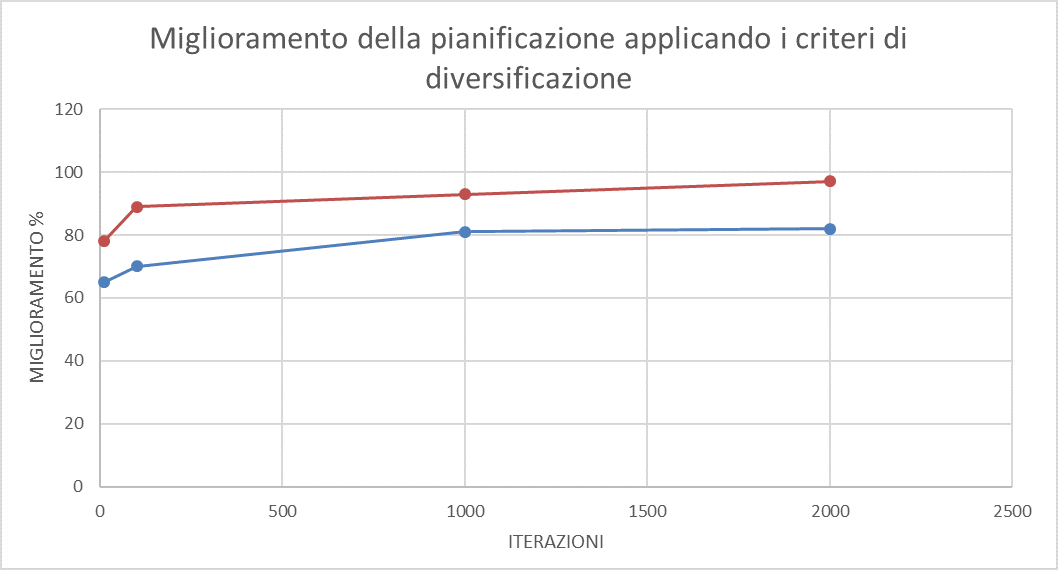
\includegraphics[width=13cm]{immagini/diversificazione.png}
	\centering
    \caption{Grafico miglioramento percentuale della soluzione della pianificazione con l'applicazione di criteri di diversificazione}
    \label{4.10}
\end{figure}

Come possiamo notare dalla \hyperref[4.10]{Figura 4.10}, vi è un miglioramento del 20\% circa della soluzione in ogni stato di esecuzione.\\
Questo evidenzia l'efficacia dei criteri di diversificazione utilizzati.
Inoltre, esaminando le soluzioni fornite pre e post inserimento dei criteri, si può notare che questi ultimi sono più efficaci se è richiesta la pianificazione di un insieme
di ordini aventi un elevato numero di pezzi, trascurando la pianificazione di molti ordini aventi un quantitativo di pezzi inferiore alla media.\\
Tali dati verranno presi in considerazione da Ergon Spa per decidere, in base alle esigenze dei clienti, quale delle due politiche di pianificazione adottare.
